\section{Aggregate results}
\label{app:aggregate-results}

\begin{figure*}[t]
  \centering
  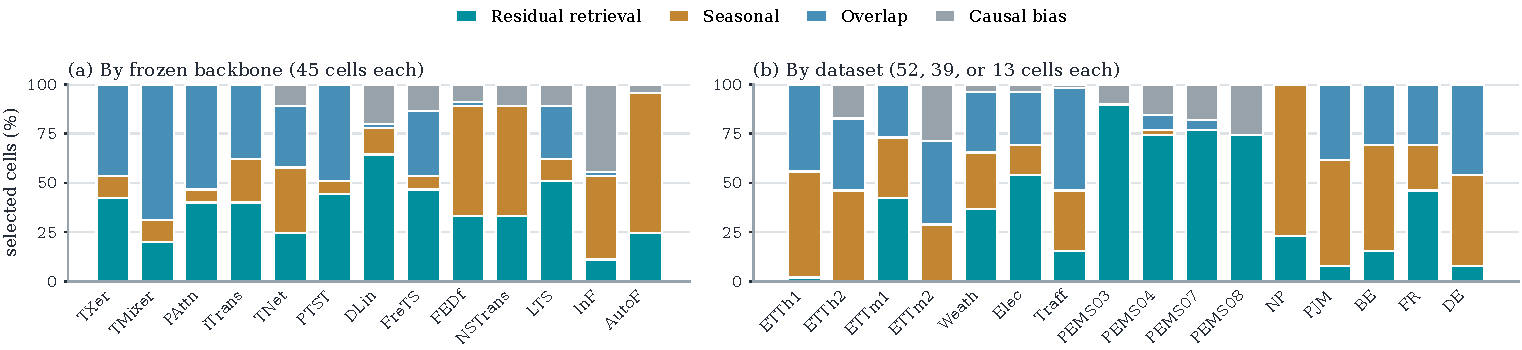
\includegraphics[width=\textwidth]{figures/selection_adaptivity.pdf}
  \caption{\textbf{Validation selects different corrections for different
  forecasters and regimes.} Share of the 585 primary settings in which each
  correction family was selected, grouped by frozen backbone (a) and by dataset
  (b). Error retrieval is chosen for 29/45 DLinear settings but 5/45 Informer
  settings, and for 35/39 PEMS03 settings but 0/52 ETTh2 settings. A fixed
  retrieval-always policy would be wrong in a large fraction of deployments.}
  \label{fig:selection}
\end{figure*}

\begin{table}[h]
\centering
\small
\caption{Primary A100 outcomes stratified by the correction family selected
on validation. This is descriptive attribution, not a
portfolio-minus-retrieval ablation.}
\label{tab:policy-attribution}
\begin{tabular}{lrr}
\toprule
Selected family & Cells & Strict wins\\
\midrule
Historical residual retrieval & 214 & 207\\
Seasonal blend & 156 & 151\\
Overlap blend & 159 & 148\\
Causal rolling bias & 56 & 56\\
Identity / static residual bias & 0 & 0\\
\midrule
Non-retrieval total & 371 & 355\\
\bottomrule
\end{tabular}
\end{table}

\begin{table*}[h]
\centering
\small
\caption{A100 configurations for the 214 cells that select historical
residual retrieval. Counts describe validation selections, not component
ablations. The search couples $(k,\tau,\lambda)$ into two settings.}
\label{tab:retrieval-configurations}
\begin{tabular}{lll}
\toprule
Quantity & Selected value & Cells\\
\midrule
Correction scale $\alpha$ & .05 / .1 / .2 / .3 / .5 & 0 / 1 / 6 / 29 / 178\\
Aggregation $(k,\tau,\lambda)$ & $(8,.1,1)$ / $(16,.3,4)$ & 151 / 63\\
Descriptor tail length & 48 / 96 / 168 & 57 / 148 / 9\\
Base-forecast features & Excluded / included & 61 / 153\\
\bottomrule
\end{tabular}
\end{table*}

All 214 selected retrieval configurations use first differences, 12 pooled
time steps, and a maximum of 16 channel groups; these fixed choices are not
ablated. Calendar features are present in 91 configurations and absent in 123,
the latter corresponding to PEMS where calendar marks are unavailable.

\begin{table*}[h]
\centering
\footnotesize
\setlength{\tabcolsep}{4pt}
\caption{A100 correction-family selections by dataset. HR is historical
residual retrieval, SB seasonal blend, OB overlap blend, and CB causal rolling
bias. Identity and static bias have zero selections on every dataset.}
\label{tab:dataset-policy-selection}
\begin{tabular}{lrrrrr@{\qquad}lrrrrr}
\toprule
Dataset & Cells & HR & SB & OB & CB &
Dataset & Cells & HR & SB & OB & CB\\
\midrule
ETTh1       & 52 & 1  & 28 & 23 & 0 &
ETTh2       & 52 & 0  & 24 & 19 & 9\\
ETTm1       & 52 & 22 & 16 & 14 & 0 &
ETTm2       & 52 & 0  & 15 & 22 & 15\\
Weather     & 52 & 19 & 15 & 16 & 2 &
Electricity & 52 & 28 & 8  & 14 & 2\\
Traffic     & 52 & 8  & 16 & 27 & 1 &
PEMS03      & 39 & 35 & 0  & 0  & 4\\
PEMS04      & 39 & 29 & 1  & 3  & 6 &
PEMS07      & 39 & 30 & 0  & 2  & 7\\
PEMS08      & 39 & 29 & 0  & 0  & 10 &
NP          & 13 & 3  & 10 & 0  & 0\\
PJM         & 13 & 1  & 7  & 5  & 0 &
BE          & 13 & 2  & 7  & 4  & 0\\
FR          & 13 & 6  & 3  & 4  & 0 &
DE          & 13 & 1  & 6  & 6  & 0\\
\bottomrule
\end{tabular}
\end{table*}

\begin{table*}[h]
\centering
\small
\setlength{\tabcolsep}{4pt}
\caption{The 23 A100 cells that do not strictly improve, grouped by dataset.
``Worst degradation'' is the largest percentage increase among reported test
metrics in that group. HR, SB, OB, and CB are defined in
Table~\ref{tab:dataset-policy-selection}.}
\label{tab:non-strict-cells}
\begin{tabular}{lrrrrrr}
\toprule
Dataset & Cells & HR & SB & OB & CB & Worst degradation\\
\midrule
Weather     & 7 & 6 & 0 & 1 & 0 & 2.45\%\\
DE          & 7 & 0 & 2 & 5 & 0 & 2.20\%\\
PEMS04      & 3 & 0 & 0 & 3 & 0 & 36.50\%\\
PEMS07      & 2 & 0 & 0 & 2 & 0 & 9.63\%\\
ETTh2       & 1 & 0 & 1 & 0 & 0 & 1.12\%\\
Electricity & 1 & 1 & 0 & 0 & 0 & 0.33\%\\
NP          & 1 & 0 & 1 & 0 & 0 & 2.64\%\\
BE          & 1 & 0 & 1 & 0 & 0 & 1.53\%\\
\midrule
Total       & 23 & 7 & 5 & 11 & 0 & 36.50\%\\
\bottomrule
\end{tabular}
\end{table*}

\begin{table}[h]
\centering
\small
\caption{A100--A10G discrepancy distribution over all 1,326 reported metric
values. Relative difference is absolute difference divided by the larger
absolute value. The frozen tolerance is
$10^{-5}+10^{-4}\max(|a|,|b|)$.}
\label{tab:hardware-consistency}
\begin{tabular}{lrr}
\toprule
Quantity & Baseline & Corrected\\
\midrule
Within tolerance & 472/1326 & 469/1326\\
Median relative difference & 0.09\% & 0.06\%\\
90th percentile & 2.95\% & 2.36\%\\
95th percentile & 5.80\% & 5.47\%\\
Maximum & 32.79\% & 28.13\%\\
\bottomrule
\end{tabular}
\end{table}

Selected methods agree in 569/585 cells, selected parameters in 529/585, and
strict-win classifications in 581/585. A100 remains the primary result; A10G
is a same-seed sensitivity check.
